\setlength\unitlength{1pt}
\begin{picture}(150,70)(70,565)  
 \put(100,200){\moocfpica} 
 \put( 0,475){\linethickness{0.4mm}\line(1,0){600}}
 \put( 0,173){\linethickness{0.4mm}\line(1,0){600}} 
 \ifEnglish
 \put(100,514){\scalefont{2.2}\bfseries\booktitleE}
 \put(100,490){\scalefont{1.6}\bfseries\booksubtitleE}
 \put(100,145){\scalefont{2.0}\bfseries Hilofumi Yamamoto}
 \put(100,130){\itshape\bfseries Ph.D.\,in Linguistics}
% \put(100,115){\itshape\bfseries Institute of Science Tokyo}
 \else
 \put(100,510){\scalefont{2.5}\bfseries\booktitleJ}
 \put(100,490){\scalefont{1.6}\bfseries\booksubtitleJ}
 \put(100,145){\scalefont{2.0}\bfseries 山 元 啓 史}
 \put(100,130){\itshape\bfseries Ph.D.\,in Linguistics}
% \put(100,115){\scalefont{1.2}\bfseries 東京科学大学}
\fi
% \put(090, 40){
\includegraphics[trim=0 0 0 0, clip, width=25mm]{img/titech12.png}}
 \put(100, 80){
\includegraphics[trim=0 0 0 0, clip, width=60mm]{img/sciencetokyologos.png}}
\end{picture}
\newpage
\ifEnglish
\noindent\booktitleE: \booksubtitleE
\else
\noindent\booktitleJ: \booksubtitleJ
\fi

 \begin{picture}(150,70)(70,300)
%  \put(60,53){\moocfpicb\ \includegraphics[height=4mm]{64px-PD-icon.png}}
  \put(60,53){\moocfpicb}
  \put(60,30){\scalefont{1.0}\pictitle}
  \put(60,20){\scalefont{0.8}\textcopyright \ \picauthor\ 2021}
%  \put(60,06){\scalefont{0.5}This work is in the public domain in its country of origin and other countries}
%  \put(60,00){\scalefont{0.5}and areas where the copyright term is the author's life plus 70 years or less.}
 \end{picture}
 
 \vfill
 
 \noindent
 \begin{tabular}[t]{rl}
  \begin{minipage}[c]{25mm}
   \fbox{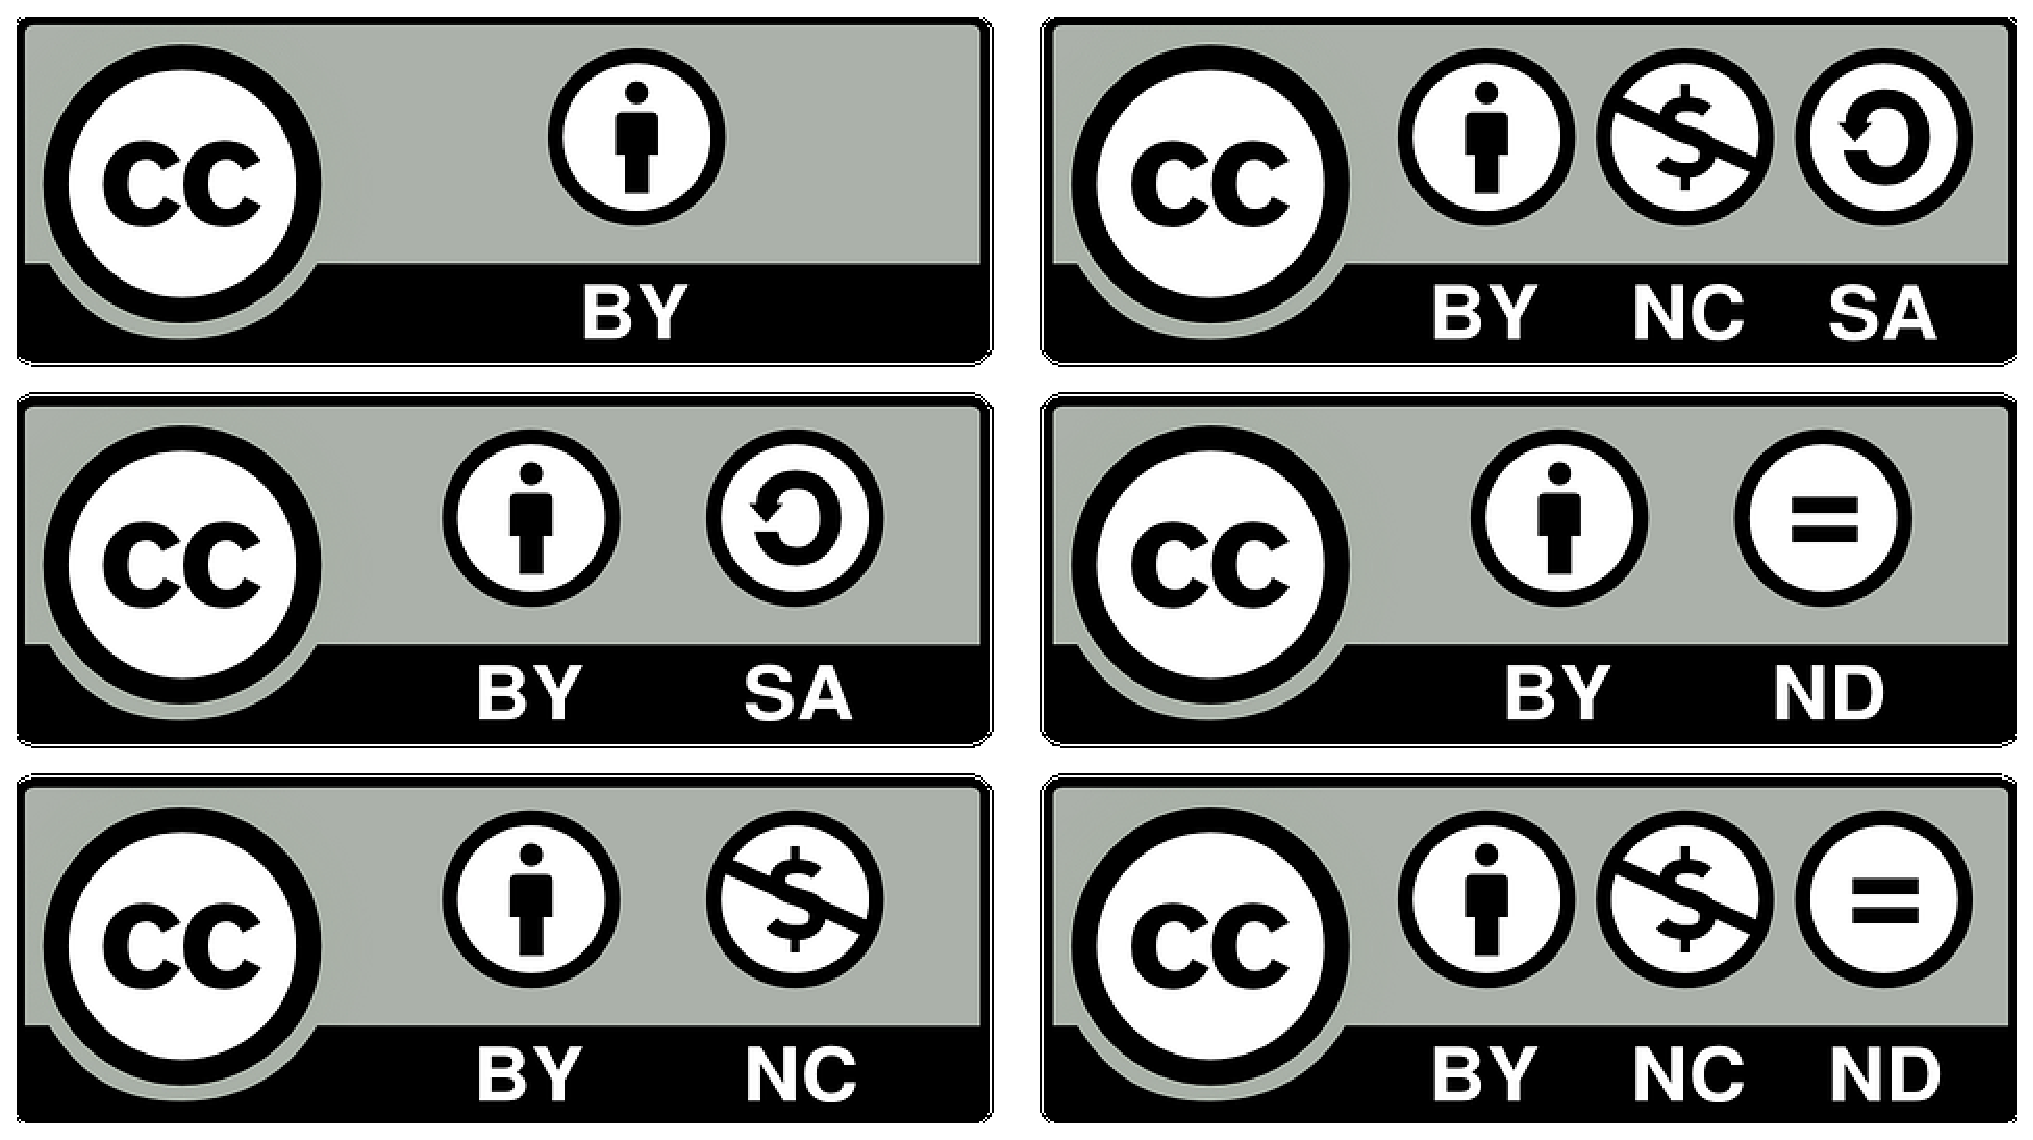
\includegraphics[trim=0 180 490 180,clip,width=20mm]{img/cclicense.eps}}
  \end{minipage} & 
  \begin{minipage}[c]{50mm}\footnotesize
   Hilofumi Yamamoto, Ph.D. \rule[-.0pt]{0pt}{8pt} \\
   Institute of Science Tokyo 
  \end{minipage}\\
 \end{tabular}
